\documentclass[11pt]{article}
\usepackage[utf8]{inputenc}
\usepackage[letterpaper, total={6in, 9in}]{geometry}
\usepackage[table,xcdraw]{xcolor}
\usepackage{hyperref}
\usepackage{adjustbox,lipsum}
\usepackage[normalem]{ulem}

\usepackage{enumitem}
\setlist{nolistsep}

\usepackage{booktabs}
\usepackage{float}
\usepackage{tabularx}
\usepackage{hyperref}
\hypersetup{
    colorlinks,
    citecolor=black,
    filecolor=black,
    linkcolor=red,
    urlcolor=blue
}
\usepackage[round]{natbib}

\graphicspath{ {Assets/} }

\title{SE 3XA3: Module Interface Specification\\Sudoku Solver}

\author{Team 08, SudoCrew
		\\ Rashad A. Bhuiyan (bhuiyr2)
		\\ Kai Zhu (zhuk2)
		\\ Stanley Chan (chans67)
}

\date{March 18, 2022}

\begin{document}
\maketitle
\tableofcontents
\newpage

\section{Module Hierarchy}
\begin{figure}[H]
\centering
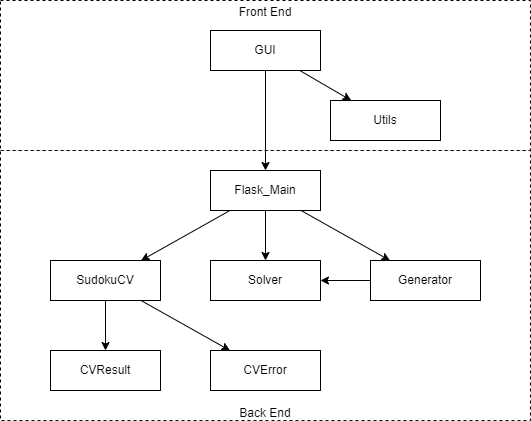
\includegraphics[width=0.7\textwidth]{useHierarchy}
\caption{Use hierarchy among modules}
\label{FigUH}
\end{figure}

% ===================================================================================

\section{SudokuCV Module}

		\subsection{Syntax}
		\subsubsection{Exported Routines}
		\begin{tabular}[width=\textwidth, pos]{|c|c|c|c|}
			
			\hline
			%	\label
			\textbf{Name}& \textbf{Inputs} & \textbf{Outputs} & \textbf{Exceptions} \\ \hline
			\_\_init\_\_ & string &  & NO\_MODEL\\ 
			recognize & image, boolean, boolean, \textcolor{red}{2D int[]} & CVResult & NO\_GRID, GRID\_SMALL, IMG\_SMALL\\
			\hline
			
		\end{tabular}
		
		\subsection{Semantics}
		\subsubsection{State Variables}
		model: The Keras machine learning model loaded for this instance of the SudokuCV.
		
		\subsubsection{Environmental Variables}
		model\_file: file path to a trained Keras machine learning model used for digit recognition. \\
		dimensions = (900, 900): specifies resolution of intermediate images during processing\\
		min\_dimensions = (200, 200): specifies minimum resolution required to process the input image\\
		
		\subsubsection{Assumptions}
		\_\_init\_\_ is called before any other access routine
		
		\subsubsection{Semantics of Exported Routines}
		\begin{itemize}
		    \item \textbf{\_\_init\_\_(model\_file)}
		\begin{itemize}
		    \item[] \textit{Input: }
			\begin{itemize}
		        \item model\_file: string; path to the trained machine learning
		    \end{itemize}	    
		    
		    \item[] \textit{Transition}: 
		    \begin{itemize}
		        \item model\_file is loaded into model state variable using Keras
		    \end{itemize}
		    
		    \item[] \textit{Exceptions}:
		    \begin{itemize}
		        \item NO\_MODEL, if no valid model file is found at model\_path
		    \end{itemize}
		\end{itemize}
		
		
		\item \textbf{recognize(image, is\_file, show\_image\textcolor{red}{, crop\_coords)}}
		\begin{itemize}
		    \item[] \textit{Input: }
			\begin{itemize}
		        \item image: a source image file path or buffer string, depending on is\_file
		        \item is\_file: optional boolean (default=True), indicates whether source is file or buffer data
		        \item show\_image: optional boolean (default=False), displays intermediary processed images for debugging
		        \item \textcolor{red}{crop\_coords: optional two dimensional integer array (default=None), an array of x-y coordinates that represent cropping points on the image}
		    \end{itemize}	    
		    
		    \item[] \textit{Output}: 
		    \begin{itemize}
		        \item CVResult object containing recognition results processed from input image.
		    \end{itemize}
		    
		    \item[] \textit{Exceptions}:
		    \begin{itemize}
		        \item NO\_GRID, if no square grid is detected in the input image.
		        \item GRID\_SMALL, if no square grid is detected in the input image.
		        \item NO\_GRID, if no square grid is detected in the input image.
		    \end{itemize}
		\end{itemize}
    \end{itemize}
			
% ===================================================================================

\section{CVResult Module}
		\subsection{Syntax}
		\subsubsection{Exported Routines}
		\begin{tabular}[width=\textwidth, pos]{|c|c|c|c|}
			
			\hline
			%	\label
			\textbf{Name}& \textbf{Inputs} & \textbf{Outputs} & \textbf{Exceptions} \\ \hline
			\_\_init\_\_ & int[], float[], image, string &  & &
			getConfidence & & 2D float[] & CV\_FAIL \\
			getConfidentResults & float & 2D int[] & CV\_FAIL \\
			saveImg & string &  & CV\_FAIL, SAVE\_FAIL\\
		    deleteImg & string & & CV\_FAIL, DEL\_FAIL\\ 
			getImage & & image & CV\_FAIL\\

			
			\hline
			
		\end{tabular}
		
		\subsection{Semantics}
		\subsubsection{State Variables}
		uuid: unique identifier for this CVResult object \\
		raw\_results: integer array of recognized digits \\
		confidence: float array of prediction confidence for each recognized digit \\
		error: error message string, empty if recognition did not experience error \\
		image: a processed image of the original input
		
		
		\subsubsection{Environmental Variables}
		N/A
		
		\subsubsection{Assumptions}
		\_\_init\_\_ is called before any other access routine. \\
		Error message string is passed into the constructor if recognition failed.
		
		\subsubsection{Semantics of Exported Routines}
		\begin{itemize}
		    \item \textbf{\_\_init\_\_(raw\_results, confidence, image, error)}
		\begin{itemize}
		    \item[] \textit{Input: }
			\begin{itemize}
		        \item raw\_results: integer list of recognized digits with 0 representing empty
		        \item confidence: float list of confidence rate from 0 (no confidence) to 1 (certain) for each result
		        \item image: processed image of the original input
		        \item error: error string description of exception encountered during recognition
		    \end{itemize}	    
		    
		    \item[] \textit{Transition}: 
		    \begin{itemize}
		        \item raw\_results and confidence lists are converted to numpy arrays and saved in respective state variables.
		        \item image and error are stored in state variables
		        \item a UUID (universally unique identifier) is generated and stored in the uuid variable
		    \end{itemize}
		    
		    \item[] \textit{Exceptions}:
		    N/A
		\end{itemize}
		
		
		\item \textbf{getConfidence()}
		\begin{itemize}
		    \item[] \textit{Input: } N/A
		    
		    \item[] \textit{Output}: 
		    \begin{itemize}
		        \item 2D float list representing confidence rates (0 to 1) for each recognized cell content
		    \end{itemize}
		    
		    \item[] \textit{Exceptions}:
		    \begin{itemize}
		        \item CV\_FAIL, if error state variable is not empty
		    \end{itemize}
		\end{itemize}

			
		\item \textbf{getConfidentResults(threshold)}
		\begin{itemize}
		    \item[] \textit{Input: } 		    
		    \begin{itemize}
		        \item threshold: float value to cut off prediction acceptance at
		    \end{itemize}
		    \item[] \textit{Output}: 
		    \begin{itemize}
		        \item 2D int list of recognized digits with confidence above threshold, 0 otherwise 
		    \end{itemize}
		    
		    \item[] \textit{Exceptions}:
		    \begin{itemize}
		        \item CV\_FAIL, if error state variable is not empty
		    \end{itemize}
		\end{itemize}
		
		\item \textbf{saveImg(directory)}
		\begin{itemize}
		    \item[] \textit{Input: } 		    
		    \begin{itemize}
		        \item directory: string path of the directory to save the image in
		    \end{itemize}
		    \item[] \textit{Transition}: 
		    \begin{itemize}
		        \item The image is saved in the specified directory using the UUID as file name
		    \end{itemize}
		    
		    \item[] \textit{Exceptions}:
		    \begin{itemize}
		        \item CV\_FAIL, if error state variable is not empty
		        \item SAVE\_FAIL, if directory does not exist or permission is denied
		    \end{itemize}
		\end{itemize}
		
		\item \textbf{deleteImg()}
		\begin{itemize}
		    \item[] \textit{Input: } 		    
		    \begin{itemize}
		        \item directory: string path of the directory to delete the image from
		    \end{itemize}
		    \item[] \textit{Transition}: 
		    \begin{itemize}
		        \item The image with the UUID as file name is deleted from the directory
		    \end{itemize}
		    
		    \item[] \textit{Exceptions}:
		    \begin{itemize}
		        \item CV\_FAIL, if error state variable is not empty
		        \item DEL\_FAIL, if file does not exist or permission is denied
		    \end{itemize}
		\end{itemize}		
		
		\item \textbf{getImage()}
		\begin{itemize}
		    \item[] \textit{Input: } N/A
		    \item[] \textit{Output}: 
		    \begin{itemize}
		        \item processed image encoded as a base64 string
		    \end{itemize}
		    
		    \item[] \textit{Exceptions}:
		    \begin{itemize}
		        \item CV\_FAIL, if error state variable is not empty
		    \end{itemize}
		\end{itemize}	
		
    \end{itemize}			
    
    % ===================================================================================

\section{CVErrors Module}
		\subsection{Syntax}
		\subsubsection{Exported Routines}
		\begin{tabular}[width=\textwidth, pos]{|c|c|c|c|}
			
			\hline
			%	\label
			\textbf{Name}& \textbf{Inputs} & \textbf{Outputs} & \textbf{Exceptions} \\ \hline
			getErrorMessage & int & string & UNDEFINED \\
			getErrors &  & dictionary & \\

			
			\hline
			
		\end{tabular}
		
		\subsection{Semantics}
		\subsubsection{State Variables}
		N/A
		
		\subsubsection{Environmental Variables}
		ERR\_MSGS: dictionary of error code matched with string descriptions
		
		\subsubsection{Assumptions}
		N/A
		
		\subsubsection{Semantics of Exported Routines}
		\begin{itemize}
		    \item \textbf{getErrorMessage(errorID)}
		\begin{itemize}
		    \item[] \textit{Input: }
			\begin{itemize}
		        \item errorID: int error code
		    \end{itemize}	    
		    
		    \item[] \textit{Output}: 
		    \begin{itemize}
		        \item string description of the error
		    \end{itemize}
		    \item[] \textit{Exceptions}:
			\begin{itemize}
		        \item UNDEFINED, if errorID is not in the ERR\_MSGS dictionary
		    \end{itemize}	  
		\end{itemize}
		
	    \item \textbf{getErrorList()}
		\begin{itemize}
		    \item[] \textit{Input: } N/A
		    
		    \item[] \textit{Output}: 
		    \begin{itemize}
		        \item returns all available error key-value pairs in the ERR\_MSGS dictionary
		    \end{itemize}
		    \item[] \textit{Exceptions}: N/A
		\end{itemize}
		
    \end{itemize}			


% ===================================================================================

\section{Solver Module}
		\subsection{Syntax}
		\subsubsection{Exported Routines}
		\begin{tabular}[width=\textwidth, pos]{|c|c|c|c|}
			
			\hline
			%	\label
			\textbf{Name}& \textbf{Inputs} & \textbf{Outputs} & \textbf{Exceptions} \\ \hline
			solve & 2D int[] & boolean &  \\
			valid & 2D int[], int[], int & boolean & INVALID\_POSITION, INVALID\_NUM \\ 
			find\_empty & 2D int[] & int[] &  \\ 
			\sout{getSolvedCoordinates} & & & \\ 
			\textcolor{red}{getUnfilledCoordinates} & 2D int[] & int[] & \\
			\textcolor{red}{solve\_randomly} & \textcolor{red}{2D int[]} & \textcolor{red}{boolean} & \\
			\textcolor{red}{validateBoard} & \textcolor{red}{2D int[]} & \textcolor{red}{boolean} & \\
			\hline
			
		\end{tabular}
		
		\subsection{Semantics}
		\subsubsection{State Variables}
		N/A
		
		\subsubsection{Environmental Variables}
		N/A
		
		\subsubsection{Assumptions}
		Input Sudoku board is a valid 9x9 2D array containing integers valued 0 to 9.
		
		\subsubsection{Semantics of Exported Routines}
		\begin{itemize}
		    \item \textbf{solve(board)}
		\begin{itemize}
		    \item[] \textit{Input: }
			\begin{itemize}
		        \item board: 2D 9x9 integer list containing digits 0 to 9, where 0 represents empty space
		    \end{itemize}	    
		    
		    \item[] \textit{Transition-Output}: 
		    \begin{itemize}
		        \item If solvable, the board is solved in place, where all 0s in the array are replaced by solution digits. The method returns True.
		        \item Returns false if the board is not solvable.
		    \end{itemize}
		    \item[] \textit{Exceptions}: N/A
		\end{itemize}
		
	    \item \textbf{valid(board, position, number)}
		\begin{itemize}
		    \item[] \textit{Input: } 
		    \begin{itemize}
		        \item board: 2D 9x9 integer list representing the cells on the game board
		        \item position: integer tuple (row, column) to specify a position on the board
		        \item number: the integer digit to test for validity at the specified position
		    \end{itemize}	  
		    \item[] \textit{Output}: 
		    \begin{itemize}
		        \item True, if number at specified position does not violate Sudoku game rules
		        \item False, if otherwise
		    \end{itemize}
		    \item[] \textit{Exceptions}:
		    \begin{itemize}
		        \item INVALID\_POSITION, if for i = 0..1 $position[i] > 8$ or $position[i] < 0 $
		        \item INVALID\_NUM, if $number > 9$ or $number < 1$
		    \end{itemize}
		\end{itemize}
		
	    \item \textbf{find\_empty(board)}
		\begin{itemize}
		    \item[] \textit{Input: } 
		    \begin{itemize}
		        \item board: 2D 9x9 integer list representing the cells on the game board
		    \end{itemize}	  
		    \item[] \textit{Output}: 
		    \begin{itemize}
		        \item (row, column) integer tuple of the position of the first empty cell on the input board.
		        \item returns empty tuple if no free cells found
		    \end{itemize}
		    \item[] \textit{Exceptions}:
		    N/A
		\end{itemize}
		
		\item \textbf{\sout{getSolvedCoordinates} \textcolor{red}{getUnfilledCoordinates}(board)}
		\begin{itemize}
		    \item[] \textit{Input: } 
		    \begin{itemize}
		        \item board: 2D 9x9 integer list representing the cells on the game board
		    \end{itemize}	  
		    \item[] \textit{Output}: 
		    \begin{itemize}
		        \item list of integer tuples with (row, column) indicating positions of empty cells to be solved
		    \end{itemize}
		    \item[] \textit{Exceptions}:
		    N/A
		\end{itemize}
		
		\item \textbf{\textcolor{red}{\textcolor{red}{solve\_randomly(board)}}}
		\begin{itemize}
		    \item[] \textit{\textcolor{red}{Input: }}
			\begin{itemize}
		        \item \textcolor{red}{board: 2D 9x9 integer list containing digits 0 to 9, where 0 represents empty space}
		    \end{itemize}	    
		    
		    \item[] \textit{\textcolor{red}{Transition-Output:}} 
		    \begin{itemize}
		        \item \textcolor{red}{If solvable, the board is solved in place, where all 0s in the array are replaced by randomly selected solution digits. The method returns True.}
		        \item \textcolor{red}{Returns false if the board is not solvable.}
		    \end{itemize}
		    \item[] \textit{\textcolor{red}{Exceptions:}} \textcolor{red}{N/A}
		\end{itemize} 
		
		\item \textbf{\textcolor{red}{validateBoard(board)}}
		\begin{itemize}
		    \item[] \textit{\textcolor{red}{Input: }}
			\begin{itemize}
		        \item \textcolor{red}{board: 2D 9x9 integer list containing digits 0 to 9, where 0 represents empty space}
		    \end{itemize}	    
		    
		    \item[] \textit{\textcolor{red}{Transition-Output:} }
		    \begin{itemize}
		        \item \textcolor{red}{Returns true if the board is completed. Also returns true if the board is incomplete but still has a solution, and solves it accordingly.}
		        \item \textcolor{red}{Returns false if the board is invalid.}
		    \end{itemize}
		    \item[] \textit{\textcolor{red}{Exceptions:}} \textcolor{red}{N/A}
		\end{itemize} 
		
    \end{itemize}
    
% ===================================================================================

\section{Generator Module}
		\subsection{Syntax}
		\subsubsection{Exported Routines}
		\begin{tabular}[width=\textwidth, pos]{|c|c|c|c|}
			
			\hline
			%	\label
			\textbf{Name}& \textbf{Inputs} & \textbf{Outputs} & \textbf{Exceptions} \\ \hline
			generateRandomValidBoard & int\sout{, int} & 2D int[] & LOW\_HINT \\ 
			hasUniqueSolution & 2D int[]\sout{, int} & boolean & INVALID\_BOARD \\ 
			\hline
			
		\end{tabular}
		
		\subsection{Semantics}
		\subsubsection{State Variables}
		N/A
		
		\subsubsection{Environmental Variables}
		N/A
		
		\subsubsection{Assumptions}
		N/A
		
		\subsubsection{Semantics of Exported Routines}
		\begin{itemize}
		    \item \textbf{generateRandomValidBoard(hints\sout{, uniquenessLikelihood})}
		\begin{itemize}
		    \item[] \textit{Input: }
			\begin{itemize}
		        \item hints: integer; number of hint digits to include in the output puzzle
		        \item \sout{uniquenessLikelihood: optional integer (default = 5); number of iterations to check for non-unique solutions. Higher values increase uniqueness of possible solutions.}
		    \end{itemize}	    
		    
		    \item[] \textit{Output}: 
		    \begin{itemize}
		        \item 2D 9x9 int list representing a newly generated Sudoku puzzle
		    \end{itemize}
		    \item[] \textit{Exceptions}: 
			 \begin{itemize}
		        \item LOW\_HINT, if the number of hints $< 24$ which results in guaranteed non-uniqueness.
		    \end{itemize}	    
		\end{itemize}
		
	    \item \textbf{hasUniqueSolution(board\sout{, attempts})}
		\begin{itemize}
		    \item[] \textit{Input: } 
		    \begin{itemize}
		        \item board: 2D 9x9 integer list representing the cells on the game board
		        \item \sout{attempts: optional integer (default = 5); number of attempts to search for a different solution.}
		    \end{itemize}	  
		    \item[] \textit{Output}: 
		    \begin{itemize}
		        \item True, if \sout{non-unique solutions are not discovered after specified number of attempts} \textcolor{red}{the Sudoku board only has one unique solution}.
		        \item False, if otherwise
		    \end{itemize}
		    \item[] \textit{Exceptions}:
		    \begin{itemize}
		        \item INVALID\_BOARD, if board is unsolvable
		    \end{itemize}
		\end{itemize}
    \end{itemize}
    
    % ===================================================================================
    
\section{GUI Module}
		\subsection{Syntax}
		\subsubsection{Exported Routines}
		\begin{tabular}[width=\textwidth, pos]{|c|c|c|c|}
			
			\hline
			%	\label
			\textbf{Name}& \textbf{Inputs} & \textbf{Outputs} & \textbf{Exceptions} \\ \hline
			constructor & & HTML GUI & &

			
			\hline
			
		\end{tabular}
		
		\subsection{Semantics}
		\subsubsection{State Variables}
		N/A
		
		\subsubsection{Environmental Variables}
		Keyboard input from user \\
		Image file upload from user \\
		HTTP request metadata from user, including browser type, version, resolution
		
		\subsubsection{Assumptions}
		Back-end application has been started.\\
		User is connecting through a major modern browser (Chrome, Edge, Firefox, Safari).\\
		
		\subsubsection{Semantics of Exported Routines}
		N/A
    
    
        % ===================================================================================

\section{Flask Main Module}
		\subsection{Syntax}
		\subsubsection{Exported Routines}
		\begin{tabular}[width=\textwidth, pos]{|c|c|c|c|}
			
			\hline
			%	\label
			\textbf{Name}& \textbf{Inputs} & \textbf{Outputs} & \textbf{Exceptions} \\ \hline
			\_\_init\_\_ & string & string & ERR\_MODEL \\
			route & HTTP GET request & HTML & ERR\_ROUTING \\ 

			
			\hline
			
		\end{tabular}
		
		\subsection{Semantics}
		\subsubsection{State Variables}
		app: Flask app instance \\
		cv: SudokuCV image recognition instance
		
		\subsubsection{Environmental Variables}
		cvModel: Keras classification model file used for image recognition \\
		home, upload, recognize, solution, play, instructions: HTML template files for HTTP response rendering
		
		\subsubsection{Assumptions}
		Hosting environment is capable of running the Flask application.
		
		\subsubsection{Semantics of Exported Routines}
		\begin{itemize}
		    \item \textbf{\_\_init\_\_(modelFile)}
		\begin{itemize}
		    \item[] \textit{Input: }
			\begin{itemize}
		        \item modelFile: Keras classification model file path
		    \end{itemize}	    
		    
		    \item[] \textit{Transition}: 
		    \begin{itemize}
		        \item An instance of SudokuCV is loaded into cv using modelFile
		        \item An instance of Flask is created and referenced in app
		    \end{itemize}
		    \item[] \textit{Exceptions}:
			\begin{itemize}
		        \item ERR\_MODEL, if specified model file path is invalid or the file cannot be loaded
		    \end{itemize}	  
		\end{itemize}
		
	    \item \textbf{route(url)}
		\begin{itemize}
		    \item[] \textit{Input: } 
		    \begin{itemize}
		        \item url: the routing path from the HTTP request
		    \end{itemize}	  
		    \item[] \textit{Output}: 
		    \begin{itemize}
		        \item url = "/" renders home HTML
		        \item url = "/upload" renders upload HTML
		        \item \textcolor{red}{url = "/game" renders difficulty selection HTML}
		        \item \sout{url = "/recognize" renders recognize HTML}
		        \item \sout{url = "/solver" renders solutions HTML}
		        \item url = "/play" renders play HTML
		        \item \sout{url = "/instructions" renders instructions HTML}
		    \end{itemize}
		    \item[] \textit{Exceptions}:
		    \begin{itemize}
		        \item ERR\_ROUTING, if url is not a valid routing address
		    \end{itemize}
		\end{itemize}
		
    \end{itemize}
    
            % ===================================================================================
    
\section{Major Revision History}
March 15, 2022 - Rough draft of sections\\
March 17, 2022 - Added MIS for SudokuCV, CVError, and CVResult \\
March 18, 2022 - Revision 0 complete \\
April 12, 2022 - Revision 1 complete, red text is new additions and strikeout text is deprecated.

			
\end{document}


